% FortySecondsCV LaTeX template
% Copyright © 2019-2022 René Wirnata <rene.wirnata@pandascience.net>
% Licensed under the 3-Clause BSD License. See LICENSE file for details.
%
% Please visit https://github.com/PandaScience/FortySecondsCV for the most
% recent version! For bugs or feature requests, please open a new issue on
% github.
%
% Contributors:
% https://github.com/PandaScience/FortySecondsCV/graphs/contributors
%
% Attributions
% ------------
% * fortysecondscv is based on the twentysecondcv class by Carmine Spagnuolo
%   (cspagnuolo@unisa.it), released under the MIT license and available under
%   https://github.com/spagnuolocarmine/TwentySecondsCurriculumVitae-LaTex
% * further attributions are indicated immediately before corresponding code


%-------------------------------------------------------------------------------
%                             ADDITIONAL PACKAGES
%-------------------------------------------------------------------------------
\documentclass[
	a4paper,
	% 9pt,
	% sidesectionsize=Large,
	% showframes,
	% vline=2.2em,
	% maincolor=cvgreen,
	% sidecolor=gray!50,
	% sidetextcolor=green,
	% sectioncolor=red,
	% subsectioncolor=orange,
	itemtextcolor=black!70,
	% sidebarwidth=0.4\paperwidth,
	% topbottommargin=0.03\paperheight,
	% leftrightmargin=20pt,
	% profilepicsize=4.5cm,
	profilepicborderwidth=2.5pt,
	profilepicstyle=profilecircle,
	profilepiczoom=1.1,
	% profilepicxshift=0mm,
	% profilepicyshift=0mm,
	% profilepicrounding=1.0cm,
	% logowidth=4.5cm,
	% logospace=5mm,
	% logoposition=before,
	% sidebarplacement=right,
	% datecolwidth=0.22\textwidth,
]{fortysecondscv}

% fine tune line spacing
% \usepackage{setspace}
% \setstretch{1.1}

% improve word spacing and hyphenation
\usepackage{microtype}
\usepackage{ragged2e}

% uncomment in case you don't want any hyphenation
% \usepackage[none]{hyphenat}

% take care of proper font encoding
\ifxetexorluatex
	\usepackage{fontspec}
	\defaultfontfeatures{Ligatures=TeX}
	% \newfontfamily\headingfont[Path=fonts/]{segoeuib.ttf} % use local font
\else
	\usepackage[utf8]{inputenc}
	\usepackage[T1]{fontenc}
\fi

% use a sans serif font as default
\usepackage[sfdefault]{ClearSans}
% \usepackage[sfdefault]{noto}

% multi-language CV XeLaTeX and polyglossia (should also work with LuaLaTeX)
% NOTE: breaks \pointskill, \membership and some spacings
% \ifxetexorluatex
% 	\usepackage{polyglossia}
% 	\newfontfamily\arabicfontsf[Script=Arabic,Scale=1.5]{Amiri}
% 	\newfontfamily\englishfontsf{Clear Sans}
% 	\setmainfont{Amiri}
% 	\setdefaultlanguage{arabic}
% 	\setotherlanguage{english}
% \fi

% enable mathematical syntax for some symbols like \varnothing
\usepackage{amssymb}

% bubble diagram configuration
\usepackage{smartdiagram}
\smartdiagramset{
	% default font size is \large, so adjust to harmonize with sidebar layout
	bubble center node font = \footnotesize,
	bubble node font = \footnotesize,
	% default: 4cm/2.5cm; make minimum diameter relative to sidebar size
	bubble center node size = 0.4\sidebartextwidth,
	bubble node size = 0.25\sidebartextwidth,
	distance center/other bubbles = 1.5em,
	% set center bubble color
	bubble center node color = maincolor!70,
	% define the list of colors usable in the diagram
	set color list = {maincolor!10, maincolor!40,
	maincolor!20, maincolor!60, maincolor!35},
	% sets the opacity at which the bubbles are shown
	bubble fill opacity = 0.8,
}

\newcommand{\intro}[3]{%
	{\Huge\color{sectioncolor}{#1}}\par%
	\setlength{\parskip}{2ex}
	{\Large\color{black!80}{#2}}\par%
	\setlength{\parskip}{1ex}
	\parbox[b]{\linewidth}{\textcolor{itemtextcolor}{#3}}
}

%-------------------------------------------------------------------------------
%                            PERSONAL INFORMATION
%-------------------------------------------------------------------------------
%% mandatory information
% your name
\newcommand{\name}{\textbf{Dr. Vanda} Farsad}
\cvname{\name}
% job title/career
\newcommand{\jobtitle}{Backend Developer} 
\cvjobtitle{\jobtitle}

%% optional information
% profile picture
\cvprofilepic{pics/vanda.pdf}
% logo picture
% \cvlogopic{pics/logo_txt.png}

% NOTE: ordering in sidebar will mimic the following order
% date of birth
\cvbirthday{August 1, 1981}
% short address/location, use \newline if more than 1 line is required
\cvaddress{Sillemstr. 35, 20257 Hamburg}
% phone number
\cvphone{+49 172 289 08 37}
% personal website
% email address
\cvmail{vanda.farsad@posteo.de}
% pgp key
% \cvkey{4096R/FF00FF00}{0xAABBCCDDFF00FF00}
% any other custom entry
% \cvsite{www.initial-commit.com}
% \cvcustomdata{\faGithub}{\href{https://github.com/VandaFarsad}{github.com/vandafarsad}}
% \cvcustomdata{\faLinkedin}{\href{https://github.com/VandaFarsad}{github.com/vandafarsad}}

%-------------------------------------------------------------------------------
%                              SIDEBAR 1st PAGE
%-------------------------------------------------------------------------------
% add more profile sections to sidebar on first page
\addtofrontsidebar{
	% include gosquare national flags from https://github.com/gosquared/flags;
	% naming according to ISO 3166-1 alpha-2 country codes
	\graphicspath{{pics/gosquared-flags/flags/flags-iso/shiny/64}}


	% \sidesection{About me}
	% \aboutme{
	% 	Hello there! With expertise in Python and experience in both DevOps and frontend technologies, 
	% 	I'm eager to assist you with the design, creation, or optimization of your web application.}

	% social network accounts incl. proper hyperlinks
	\sidesection{Links}
		\begin{icontable}[1.5]{2.5em}{1em}
			\social{\faGlobe}
				{https://www.initial-commit.com}
				{Home Page}
			\social{\faLinkedin}
			{https://www.linkedin.com/in/vanda-farsad-4b98321a5/}
			{LinkedIn}
			\social{\faGithub}
			{https://github.com/VandaFarsad}
			{Github}
		\end{icontable}
		
	\sidesection{Stack}
	\begin{figure}\centering
		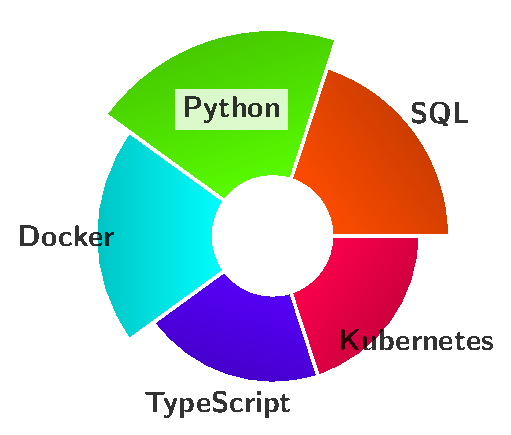
\includegraphics[scale=0.65]{pics/diagrams/stack.pdf}
	\end{figure}

	\sidesection{Frameworks}
	\pointskill{}{Django}{5}
	\pointskill{}{Flask}{3}
	\pointskill{}{React}{2}
	\pointskill{}{Next.js}{2}

	\sidesection{Languages}
	\pointskill{\flag{DE.png}}{German}{5}
	\pointskill{\flag{GB.png}}{English}{3}
	\pointskill{\flag{IR.png}}{Persian}{2}

% 	\sidesection{Hard Skills}
% 		\skill{\faBalanceScale}{Sleeping almost all day}
% 		\skill{\faSitemap}{Eating a lot of bamboo sprouts}
% 		\skill{\faGraduationCap}{Relaxing rest of the day}

	% \sidesection{Soft Skills}
% 		\pointskill{\faHome}{Looking Cute}{4}[4]
% 			\skill[1.8em]{\faCompress}{No need to specify further}
% 		\pointskill{\faChild}{Chillin' hard}{3}[4]
% 			\skill[1.8em]{\faCompress}{On a tree}
% 			\skill[1.8em]{\faCompress}{In the grass}

}


%-------------------------------------------------------------------------------
%                              SIDEBAR 2nd PAGE
%-------------------------------------------------------------------------------
\definecolor{pastelgreen}{HTML}{D7ECD9}
\definecolor{pastelpurple}{HTML}{D5D6EA}
\definecolor{pastelorange}{HTML}{F5D5CB}
\definecolor{pastelyellow}{HTML}{F6F6EB}

\addtobacksidebar{
	\sidesection{About Me}
	\aboutme{
		The giant panda is a terrestrial animal and primarily spends its life
		roaming and feeding in the bamboo forests of the Qinling Mountains and in
		the hilly province of Sichuan.
	}

	\sidesection{Diagrams}
	\begin{sidebarminipage}
		\chartlabel[pastelgreen]{Bubble}
		\chartlabel[pastelgreen]{Diagrams}
		\chartlabel[pastelpurple]{with}
		\chartlabel[pastelpurple]{proper}
		\chartlabel[pastelorange]{overflow}
		\chartlabel[pastelorange]{protection}
		\chartlabel[pastelyellow]{for}
		\chartlabel[pastelyellow]{labels}
	\end{sidebarminipage}

	\begin{figure}\centering
		\smartdiagram[bubble diagram]{
			\textcolor{white}{\textbf{Being a}} \\
			\textcolor{white}{\textbf{Panda}}, % center bubble
			\textcolor{black!90}{Eating},
			\textcolor{black!90}{Sleeping},
			\textcolor{black!90}{Rolling},
			\textcolor{black!90}{Playing},
			\textcolor{black!90}{Chilling}
		}
	\end{figure}

	\chartlabel{Wheel Chart}

	\wheelchart{3.7em}{2em}{%
	20/3em/maincolor!50/Chill,
	15/3em/maincolor!15/Play,
	30/4em/maincolor!40/Sleep,
	20/3em/maincolor!20/Eat
	}

	\sidesection{Barskills}
	\barskill[1ex]{\faSkyatlas}{Wearing asian rice hats}{60}
	\barskill[2ex]{\faImage}{Playing Chess}{30}
	\barskill[3ex]{\faMusic}{Playing the bamboo flute}{50}

	\sidesection{Memberships}
	\begin{memberships}
		\membership[4em]{pics/logo.png}{PandaScience.net}
		\membership[4em]{pics/logo.png}{Some longer text spanning over more than
			only one line}
	\end{memberships}
}


%-------------------------------------------------------------------------------
%                         TABLE ENTRIES RIGHT COLUMN
%-------------------------------------------------------------------------------
\begin{document}

\makefrontsidebar

\newgeometry{left=3in, right=0.25in, top=0.75in, bottom=0.5in}

\intro{\name}{\jobtitle}{
	Hey! With my expertise in Python and a versatile understanding of DevOps and frontend technologies, I'm excited to
	contribute to the design, development, and optimization of your web applications. With a keen eye for detail and a
	commitment to delivering high-quality solutions, I aim to craft code that is both maintainable and testable.\\
	Let's collaborate to create innovative and efficient solutions that align with your organization's goals.
}

\cvsection{Working Experience}
\begin{cvtable}[3]
	\cvitem{since 2020}{Freelance Backend Developer}{Orendt Studios}{Development, testing and maintenance of Django-based
		web applications, CI/CD pipelines and frontend frameworks.
		Managed the full lifecycle of development projects, from strategic planning to successful implementation
		and taking responsibility for timelines.\\\\
		Backend Technologies: Python (Django, Flask)\\
		Frontend Technologies: Typescript (Next.js, React)\\
		CI/CD Tools: Docker, Kubernetes, Gitlab}
	\cvitem{2019 -- 2019}{Senior Consultant Biostatistics}{Ecker+Ecker}{
		In addition, project management.}
	\cvitem{2017 -- 2019}{Consultant Biostatistics}{Ecker+Ecker}{
		Developed Python software for various applications, conducted data analysis using Python and R, evaluated
		clinical trials, provided statistical guidance to customers and team members, and delivered statistics training.
	}
	\cvitem{2008 -- 2010}{Research assistant}{Fraunhofer-Institute LBF}{Executed method implementations using
		Matlab/Simulink and conducted numerical simulations for comprehensive analysis.}
\end{cvtable}


\cvsection{Education}

\begin{cvtable}[1.5]
	\cvitem{2014 -- 2017}{Ph.D $\bullet$ Mathematics (\normalfont{cum laude})}{Universit\"at Hamburg}
	{Thesis: \emph{The symplectic fermion ribbon quasi-Hopf algebra and the $SL(2,\mathbb{Z})$-action on its centre.}
		\footnote{\href{https://doi.org/10.1016/j.jalgebra.2018.12.012}{
				Journal of Algebra. 522. 10.1016/j.jalgebra.2018.12.012}, 2017.}
		\footnote{\href{https://doi.org/10.1016/j.aim.2022.108247}{
				Advances in Mathematics. 400. 10.1016/j.aim.2022.108247}, 2022.}
	}
	\cvitem{2009 -- 2013}{Master of Science $\bullet$ Mathematics ($\varnothing\, 1,5$)}{TU Darmstadt}
	{Focus: Geometry, Nuclear Physics and Operator Algebra}
	\cvitem{2005 -- 209}{Diploma $\bullet$ Applied Mathematics ($\varnothing\, 1,3$)}{Hochschule Darmstadt}
	{Focus: Numerical Mathematics and Computer Science (C\texttt{++})}
\end{cvtable}

% \cvsection{Publications}
% \begin{cvtable}
% 	\cvpubitem{Cooking: 100 recipes for lazy Pandas}{Me and My Panda Friends}
% 	{Panda's Culinary World}{2010}
% 	\cvpubitem{Pandastasia}{Still Me}{Bamboo Books Assoc.}{2005}
% \end{cvtable}

% \cvsection{Awards}
% \begin{cvtable}
% 	\cvitem{2010 -- now}{Panda of the Year}{Panda World Forum}{}
% 	\cvitem{2005 -- now}{Face of World Wide Fund for Nature}{WWF}{}
% 	\cvitem{2000}{Winner of Bamboo Sprouts Eating Contest}{Bamboo Society}{}
% \end{cvtable}


% \cvsection{Extra-Curricular Activities}
% \begin{cvtable}
% 	\cvitemshort{Relaxing}{Master the fine art of relaxing everywhere}
% 	\cvitemshort{Music}{Playing the bamboo flute in the 1st Panda Orchestra}
% 	\cvitemshort{Education}{Teaching young pandas to be more panda-like}
% \end{cvtable}


% \newpage
% \makebacksidebar
% % \newgeometry{
% % 	top=\topbottommargin,
% % 	bottom=\topbottommargin,
% % 	right=\leftrightmargin,
% % 	left=\leftrightmargin
% % }

% \cvsection{section}
% \cvsubsection{Subsection}
% \begin{cvtable}
% 	\cvitem{<dates>}{<cv-item title>}{<location>}{<optional: description>}
% \end{cvtable}

% \cvsection{cvitem}
% \cvsubsection{Multi-line with longer description}
% \begin{cvtable}
% 	\cvitem{date}{Description}{location}{Some longer and more detailed
% 		description, that takes two lines of space instead of only one.}
% 	\cvitem{date}{Description}{location}{Some longer and more detailed
% 		description, that takes two lines of space instead of only one.}
% 	\cvitem{date}{Description}{location}{Some longer and more detailed
% 		description, that takes two lines of space instead of only one.}
% \end{cvtable}

% \cvsubsection{One-line without description}
% \begin{cvtable}
% 	\cvitem{Award}{One-line description}{Sponsor}{}
% 	\cvitem{Award}{One-line description}{Sponsor}{}
% 	\cvitem{Award}{One-line description}{Sponsor}{}
% \end{cvtable}

% \cvsection{cvitemshort}
% \cvsubsection{One-line}
% \begin{cvtable}
% 	\cvitemshort{Key}{Some further description}
% 	\cvitemshort{Key}{Some further description}
% 	\cvitemshort{Key}{Some further description}
% \end{cvtable}

% \cvsubsection{Multi-line with longer description}
% \begin{cvtable}
% 	\cvitemshort{Key}{Some further description. Can fill even more than
% 		only one single line while still keeping the correct indendation level.}
% 	\cvitemshort{Key}{Some further description. Can fill even more than
% 		only one single line while still keeping the correct indendation level.}
% 	\cvitemshort{Key}{Some further description. Can fill even more than
% 		only one single line while still keeping the correct indendation level.}
% \end{cvtable}

% \cvsection{cvpubitem}
% \begin{cvtable}
% 	\cvpubitem{Publication title}{Authors}{Journal}{Year}
% 	\cvpubitem{Publication title}{Authors}{Journal}{Year}
% 	\cvpubitem{Publication title that is spanning over multiple lines and still
% 		does not look too bad}{Authors}{Journal}{Year}
% \end{cvtable}

% \cvsignature

\end{document}
